\documentclass[14pt]{beamer}
\usetheme{Antibes}
\definecolor{myOrange}{RGB}{255,73,37}
\setbeamercolor*{palette primary}{fg=myOrange}
\setbeamercolor*{palette secondary}{fg=myOrange,bg=white}
\setbeamercolor*{palette tertiary}{bg=myOrange,fg=white}
\setbeamercolor*{titlelike}{parent=palette primary}
\setbeamercolor*{itemize item}{fg=myOrange}
\setbeamercolor{block title example}{bg=myOrange} 
\setbeamercolor{section in toc}{fg=black}
\setbeamertemplate{sections/subsections in toc}[sections numbered]
\setbeamercolor{section number projected}{bg=myOrange,fg=yellow}
\setbeamertemplate{footline}[frame number]
\setbeamertemplate{frametitle}{
  \begin{centering}
  \insertframetitle
    \par
    \end{centering}
}
\setbeamertemplate{itemize item}{\textbullet}

\usepackage{amsmath}
\usepackage[english]{babel}
\usepackage{hyperref}
\usepackage{ulem}
\logo{
\includegraphics[width=1cm]{logo.png}}
\newcommand\B{\rule[-1.7ex]{0pt}{0pt}}

\setcounter{tocdepth}{1}

\begin{document}
\title{Lambda Expressions in Java 8 \\ Sessions Report}
\author{Arkady Galyash}
\institute{dxChartPro}
\date{\today}

\newcommand{\smaller}[1] {
  {\scriptsize {#1}}
}
\def\colored#1{\textcolor{myOrange}{#1}}

\frame{\titlepage}

\frame
{\frametitle{Agenda}
  \tableofcontents[1]
}

\section{Lambda Intro}
\subsection{Why Lambda Project is so popular?}
\frame{\frametitle{Why Lambda Project is so popular?}
  \begin{itemize}
    \item Huge language and library improvements
    \item Perhaps the biggest upgrade ever to the Java programming model
    \item We want to treat code as data
  \end{itemize}
}

\subsection{What is a Lambda Expression?}
\frame{\frametitle{What is a Lambda Expression?}
  Lambda expression(closure) is an anonymous method
      \begin{itemize}
        \item has an argument list, a return type, a body
	\item can refer values from the enclosing lexical scope
	\item not a member of a class - just free-floating expression
      \end{itemize}
}

\frame{\frametitle{Who needs Lambda Expressions?}
  \begin{itemize}
    \item C++ added them
    \item C\# added them 
    \item Scala, Groovy, Clojure, Kotlin, ...
  \end{itemize}
  \begin{exampleblock}{} 
    {In another thirty years people will laugh at anyone who tries to invent a language without closures, just as they'll laugh now at anyone who tries to invent a language without recursion.}
    \vskip 3mm 
    \hspace*\fill{\small--- Mark Jason Dominus, ``The Perl Review''} 
  \end{exampleblock}
}

\subsection{How Lambda Expression looks like?}
\frame{\frametitle{How Lambda Expression looks like?}
  \begin{center}
    \large Talk is cheap. Show me the code.
  \end{center}
}

\subsection{What have been done?}
\frame{\frametitle{What have been done?}
  JSR-335 =
    \begin{itemize}
      \item Lambda Expression
      \item Interface Evolution
      \item Bulk Collection Operations
    \end{itemize}
}

\section{Lambda Expression}
\frame{\frametitle{Study calculation example}
  \begin{itemize}
    \item Chart with some studies
    \item Study can be calculated
    \item Some studies are visible and some are hidden
    \item New bars have come - we need to recalculate studies
  \end{itemize}
}

\frame{\frametitle{What is changed?}
  \begin{itemize}
    \item Library is in control(parallelism, laziness)
    \item Behavior have been passed into the API as data
    \item Internal iteration
    \item More what, less how
  \end{itemize}
}

\frame{\frametitle{How much syntax sugar do we have?}
  \begin{itemize}
    \item Remove curly brackets and return for single expression
    \item Type argument inference
    \item Method reference \\
    \texttt{Classname::methodName}
    \item Expression method reference \\
    \texttt{Expression::methodName}
    \item Effectively final local variables
  \end{itemize}
}

\frame{\frametitle{What about type?}
  \begin{itemize}
    \item Now we are using single-method interfaces to represent functions: \\ Runnable, Comparator, ActionListener
    \item Let's give these a name: functional interfaces
    \item We need more functional interfaces: \\ Predicate, Block, etc.
    \item Everything we wrote before will work with lambda for free
  \end{itemize}
}

\section{Interface Evolution}
\frame{\frametitle{Interface evolution}
  \begin{center}
    \large \texttt{Collection::forEach\\(Block$<$? super E$>$)} \\ What is this?
  \end{center}
}

\begin{frame}[t]
\frametitle{Interface inheritance rules}
  $ $
  \begin{itemize}
    \item ArrayList \only<1>{VS}\only<2->{\colored{$>$}} List  \onslide<2->{\colored{"superclass always wins"}} \\ $ $
    \onslide<3->{\item List} \only<3>{VS}\only<4->{\colored{$>$}} \onslide<3->{Collection} \onslide<4->{\colored{"subtype wins"}} \\ $ $
    \onslide<5->{\item List} \only<5>{VS}\only<6>{\colored{==}} \onslide<5->{Set} \only<6>{\colored{write your implementation}}
  \end{itemize}
\end{frame}

\frame{\frametitle{Diamond problem}
  \begin{center}
    
\includegraphics[width=0.99\textwidth]{diamonds.png}
  \end{center}
}

\section{Library Changes}
\subsection{java.util.Collection}
\frame{\frametitle{java.util.Collection}
  \texttt{
  \begin{itemize}
    \item \texttt{void \colored{forEach}(Block$<$? super E$>$)} \\
    \item \texttt{boolean \colored{removeIf}(Predicate$<$? super E$>$)} \\
    \item \texttt{\colored{Stream$<$E$>$ stream()}}
    \item \texttt{\colored{Stream$<$E$>$ parallel()}}
  \end{itemize}
  }
}

\subsection{java.util.streams.Stream}
\frame{\frametitle{java.util.stream.Stream}
  Methods for FP-lovers
    \texttt{
  \begin{itemize}
    \item $<$R$>$ Stream$<$R$>$ \colored{map}(Mapper$<$? super T, ? extends R$>$ mapper);
    \item $<$R$>$ Stream$<$R$>$ \colored{flatMap}(FlatMapper$<$? super T, R$>$ mapper);
    \item Stream$<$T$>$ \colored{filter}(Predicate$<$? super T$>$ predicate);
  \end{itemize}
    }
}

\frame{\frametitle{java.util.stream.Stream \#2}
  Terminal methods
  \texttt{
  \begin{itemize}
    \item $<$U$>$ U \colored{fold}(Factory$<$U$>$ baseFactory, \\
	             Combiner$<$U, T, U$>$ reducer, \\
		     BinaryOperator$<$U$>$ combiner);
    \item T \colored{reduce}(T base, BinaryOperator$<$T$>$ op);
    \item Optional$<$T$>$ \colored{reduce}(BinaryOperator$<$T$>$ op);
    \item $<$A extends Destination$<$? super T$>$$>$ A \colored{into}(A target);
  \end{itemize}
  }
}

\frame{\frametitle{Parallel Stream}
  \begin{itemize}
    \item \colored{Stream$<$E$>$ parallel()}
    \item Over fork/join framework
    \item \colored{java.util.streams.Spliterator} provides the ability to decompose an aggregate data structure and to iterate over the elements of the aggregate
  \end{itemize}
}

\section{Lambda in JVM}
\frame{\frametitle{Lambda in JVM}
  \begin{center}
    
\includegraphics[height=0.8\textheight]{deeper.png}
  \end{center}
}

\frame{\frametitle{Lambda is just sugar?}
  We could say that a lambda is "just" an inner class instance. \\
    \colored{Pros}:
  \begin{itemize}
    \item Simple, quick and dirty
    \item We use that already worked
  \end{itemize}
}

\frame{\frametitle{Lambda is just sugar?}
  We could say that a lambda is "just" an inner class instance. \\
  \colored{Cons}:
  \begin{itemize}
    \item One class per lambda expression(performance issues)
    \item Whatever we do becomes a binary representation for lambdas in Java(forever)
  \end{itemize}
}

\frame{\frametitle{JVM Bytecode}
  \begin{center}
    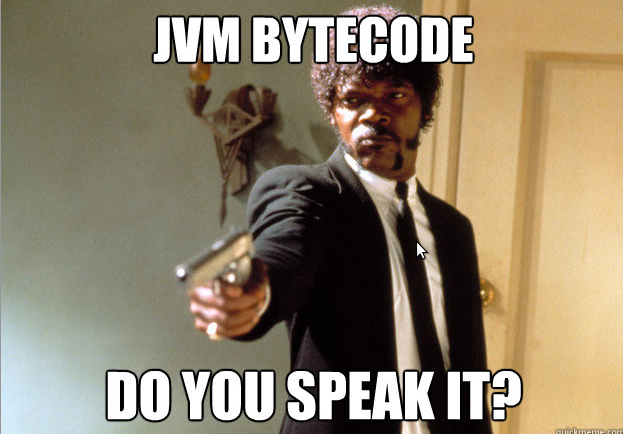
\includegraphics[height=0.8\textheight]{do_you.png}
  \end{center}
}

\frame{\frametitle{Bytecode invocation modes}
  Prior to Java 7, the JVM had four bytecodes for method invocation
  \begin{itemize}
    \item invokestatic - for static methods
    \item invokevirtual - for class methods
    \item invokeinterface - for interface methods
    \item invokespecial - for everything else
  \end{itemize}
}

\frame{\frametitle{java.lang.invoke.MethodHandle}
  \begin{itemize}
    \item From Java7
    \item Typed, directly executable reference to an underlying method or similar low-level operation, with optional transformations of arguments or return values
    \item Can be saved into runtime constant pool of the class and loaded with LDC
    \item Sounds like lambda
  \end{itemize}
}

\frame{\frametitle{java.lang.invoke.MethodHandle}
  \begin{exampleblock}{}
  list.removeAll(...)
  \end{exampleblock}
  \begin{exampleblock}{}
  private static boolean lambda\$1(...) \{ ... \}
  \end{exampleblock}
  \begin{exampleblock}{}
  MethodHandle mh = LDC[lambda\$1];\\
  mh = mh.insertArguments(mh, ...); \\
  list.removeAll(mh);
  \end{exampleblock}
}

\frame{\frametitle{java.lang.invoke.MethodHandle}
  \colored{Cons}:
  \begin{itemize}
    \item Signature will be \\
      void removeAll(MethodHandle predicate)
    \item Erasure worse than with generics(all lambda are the same)
    \item Whatever we do becomes a binary representation for lambdas in Java(forever)
  \end{itemize}
}

\frame{\frametitle{invokedynamic}
  \begin{itemize}
    \item From Java7
    \item Let some "language logic" determinate call target
    \item Language and VM become partners in flexible and efficient method dispatch
    \item java.lang.invoke.CallSite
  \end{itemize}
}

\frame{\frametitle{indy and Lambda}
  \begin{itemize}
    \item indy lets us separate the binary representation of lambda creation in the bytecode from the mechanics of evaluating the lambda expression at runtime
    \item Instead of generating bytecode to create the object that implements the lambda expression (such as calling a constructor for an inner class), we describe a recipe for constructing the lambda, and delegate the actual construction to the language runtime
  \end{itemize}
}

\frame{\frametitle{java.lang.invoke.LambdaMetafactory}
  \begin{itemize}
    \item Bootstrap for the lambda factory selects the translation strategy
    \item The runtime implementation choice is hidden behind a standardized API for lambda construction(invokedynamic)
  \end{itemize}
}

\frame{\frametitle{java.lang.invoke.LambdaMetafactory}
  \begin{center}
    \large Talk is cheap. Show me the \sout{ code } bytecode.
  \end{center}
}

\frame{\frametitle{Desugaring Lambda}
  \begin{itemize}
    \item For "stateless" lambda - generate private static method at the same class with the signature of SAM
    \item For lambda capturing immutable values - generate private static method at the same class with the signature of SAM + additional captured parameters
    \item For lambda with this, super, etc. - generate private method of the same class with the signature of SAM
  \end{itemize}
}

\subsection{Lambda Serialization}
\frame{\frametitle{Lambda Serialization}
  \begin{center}
    
\includegraphics[width=0.9\textwidth]{serialization.png}
  \end{center}
}
\frame{\frametitle{Lambda Serialization}
  \begin{itemize}
    \item Dynamic translation strategy mandates a dynamic serialization strategy
    \item The serialized form(\colored{java.lang.invoke.SerializedLambda}) would have to contain all the information needed to recreate the object through the metafactory
  \end{itemize}
}

\section{Links}
\subsection{HowTo play with Lambda?}
\frame{\frametitle{HowTo play with Lambda?}
  \begin{itemize}
    \item \href{http://openjdk.java.net/projects/lambda/}{Project Lambda}
    \item \href{http://hg.openjdk.java.net/lambda/lambda}{hg repository}
    \item \href{http://jdk8.java.net/lambda/}{Binary snapshots}
    \item -XDlambdaToMethod
  \end{itemize}
}

\subsection{What to read about Lambda?}
\frame{\frametitle{What to read about Lambda?}
  \begin{itemize}
    \item \href{http://cr.openjdk.java.net/~briangoetz/lambda/lambda-state-4.html}{State of the Lambda v4}
    \item \href{http://cr.openjdk.java.net/~briangoetz/lambda/Defender\%20Methods\%20v4.pdf}{Defender methods v4}
    \item \href{http://cr.openjdk.java.net/~briangoetz/lambda/collections-overview.html}{State of the Lambda: Libraries Edition}
    \item \href{http://cr.openjdk.java.net/~briangoetz/lambda/lambda-translation.html}{Translation of Lambda Expressions}
    \item CON4862, CON6080
  \end{itemize}
}

\frame{
  \begin{center}
    Thank You!
  \end{center}
}
\end{document}
